\documentclass[../main.tex]{subfiles}

\begin{document}

\section{Results}

Presented here are the results of investigations into different advanced microscopy techniques and development and application of image processing tools to determine CheZ fraction. Further to this we present the adaptation of our existing library of protein fusions for homo-FRET, and the preliminary work towards using the technique to directly measure density of CheZ in the chemotactic cluster.

\subsection{Localisation Microscopy (GSD)}

GSD is a technique that does not have stringent requirements on fluorophores, as compared to STORM/PALM like techniques. As such, we were able to use existing strains in a Leica demo unit at a workshop run by Leica (Figure~\ref{fig:results:palm}).

\begin{figure}[h!]
\begin{center}
\subfloat[Epifluorescent image]{
	\setlength\fboxsep{0pt}
	\setlength\fboxrule{1pt}
	\fbox{
		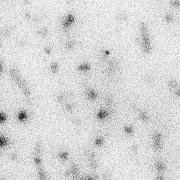
\includegraphics[height=.48\textwidth]{\docroot results/figs/PALMOriginal}
	}
	\label{fig:results:palm:original}
}
\subfloat[GSD reconstruction]{
	\fbox{
		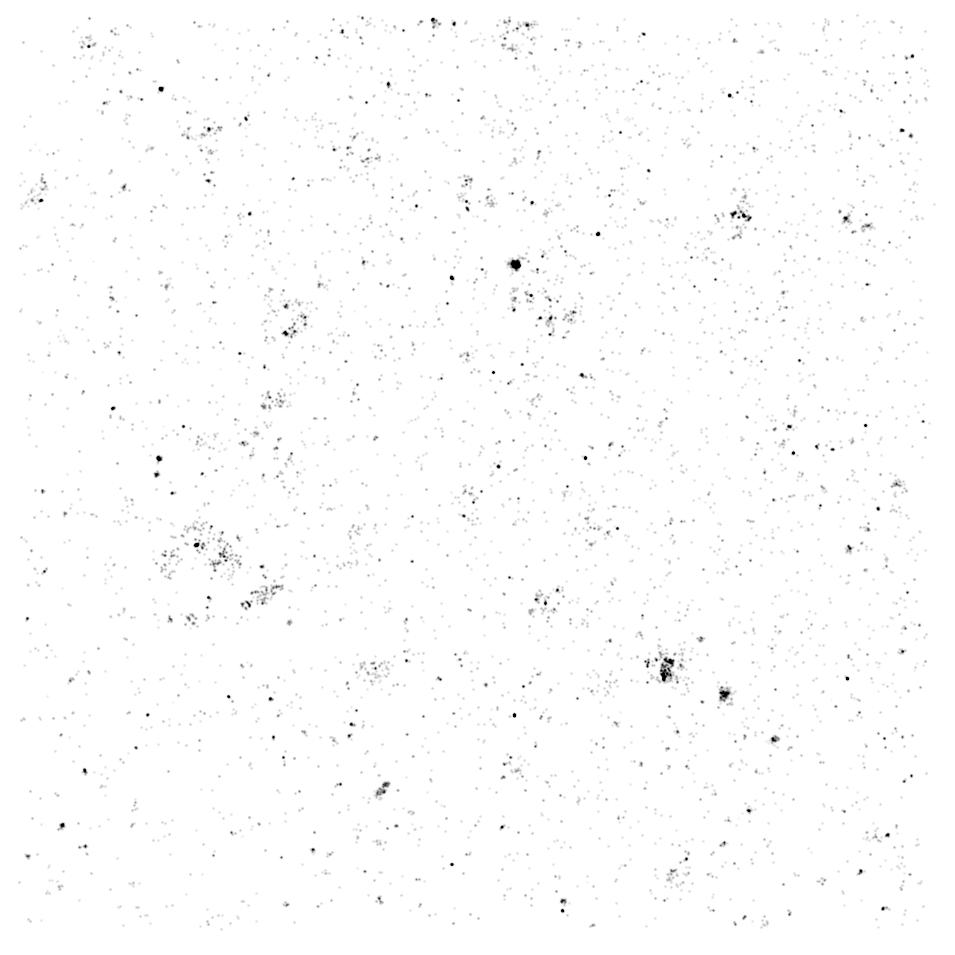
\includegraphics[height=.48\textwidth]{\docroot results/figs/PALMReconstruction}
	}
	\label{fig:results:palm:reconstruction}
}
\caption[GSD reconstruction]{GSD reconstruction of image. From 17990 frames in non-optimal medium.}
\label{fig:results:palm}
\end{center}
\end{figure}
\newpage
\subsection{STED}

STED offers an improved resolution using an imaging technique similar to confocal microscopy - direct, pixel by pixel imaging of the cell (Figure~\ref{fig:results:sted}).

\begin{figure}[h!]
\begin{center}
\subfloat[Confocal microscopy]{
	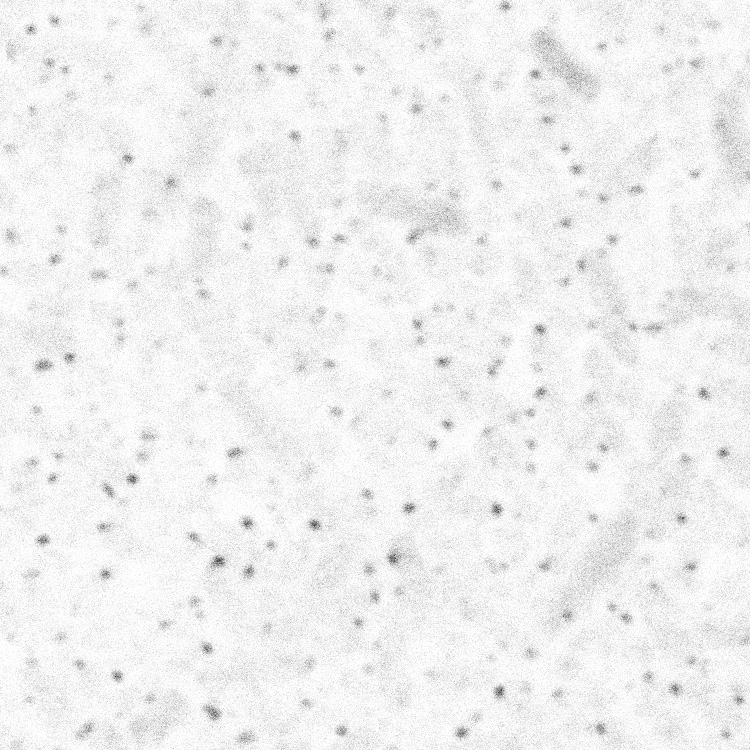
\includegraphics[width=0.45\textwidth]{\docroot results/figs/sted-con}
	\label{fig:results:sted:con}
}
\subfloat[STED Microscopy]{
	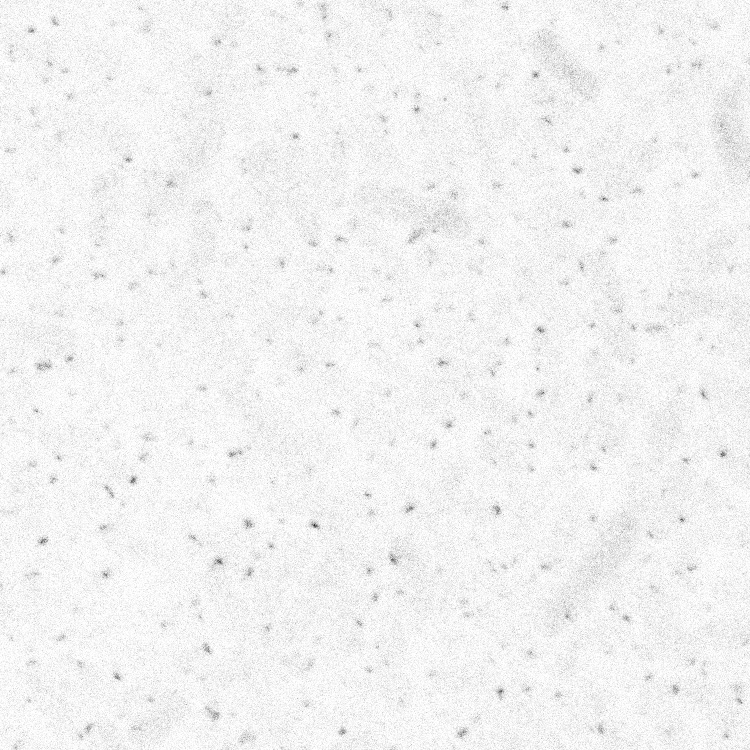
\includegraphics[width=0.45\textwidth]{\docroot results/figs/sted-sted}
	\label{fig:results:sted:sted}
}
\caption[STED microscopy]{STED Microscopy. Both images are of the same sample of KL1005 taken simultaneously. Colours inverted and contrasted adjusted identically, and cropped for clarity.}
\label{fig:results:sted}
\end{center}
\end{figure}
\newpage


\subsection{Image Processing}
\label{sec:results:imageprocessing}

\subsubsection{Cluster Detection}
One basic objective was to determine the fraction of CheZ in the chemotaxis protein clusters on the poles of the \ecoli. At the start of the project there were existing scripts that identified clusters through threshold detection. Whilst this performed reasonably well on high contrast images, it struggled on more noisy images, and could not identify cells with more than one cluster, or none at all.

A brief description of the two scripts written to identify the size and density of clusters follows - for more details see appendix~\ref{sec:scripts}.

\paragraph{Cell Finder}\ \\
This script outputs a black and white map of all objects in an image that can be identified as cells, subject to a set of user-defined constraints (size, shape, brightness etc.). This process is visualised in Figure~\ref{fig:imageprocessing:celldetection}.

\begin{figure}[p]
\begin{center}
\subfloat[Raw greyscale image]{
	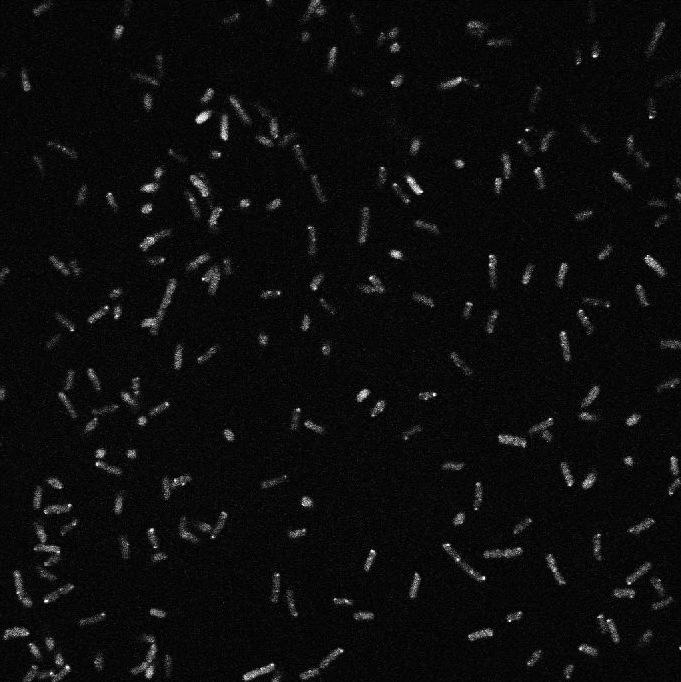
\includegraphics[scale=0.64]{\docroot results/figs/slide1}
	\label{fig:imageprocessing:raw}
}
\subfloat[Edge detection]{
	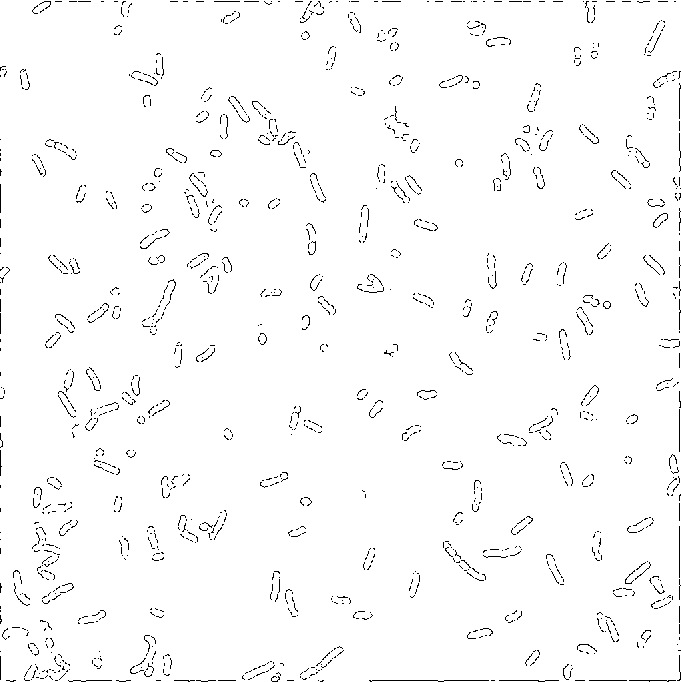
\includegraphics[scale=0.64]{\docroot results/figs/slide2}
	\label{fig:imageprocessing:edges}
}\\
\subfloat[Detected Cells]{
	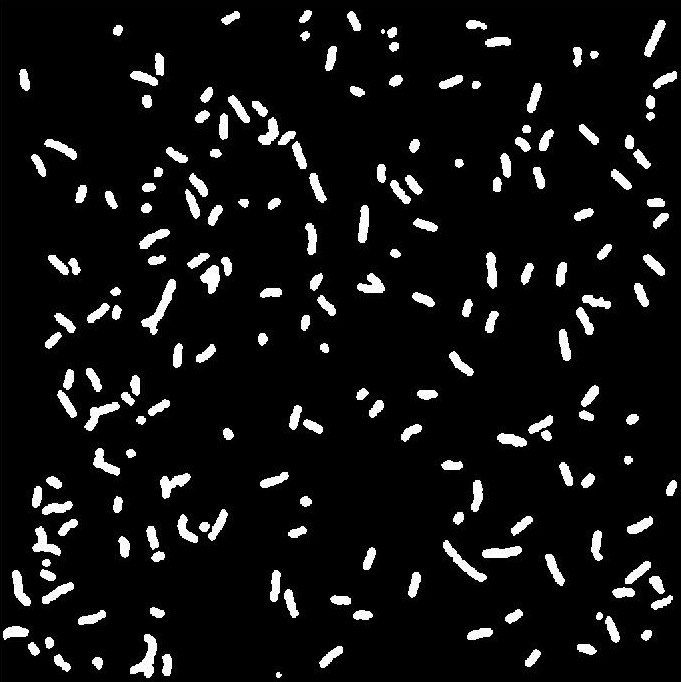
\includegraphics[scale=0.64]{\docroot results/figs/slide3}
	\label{fig:imageprocessing:cells}
}
\subfloat[Accepted Cells]{
	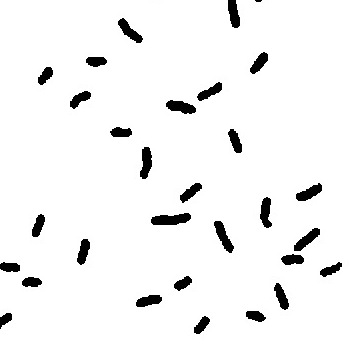
\includegraphics[scale=0.64]{\docroot results/figs/slide4}
	\label{fig:imageprocessing:accepted}
}
\caption[Depiction of cell detection]{\subref{fig:imageprocessing:raw} The original greyscale image. \subref{fig:imageprocessing:edges} To generate the mask of cells, the script first performs edge detection using the Canny method~\citep{canny}. This is particularly effective for detecting edges in noisy images. The lines are then thickened and the gaps closed to give the outline of cells. \subref{fig:imageprocessing:cells} The outlines are filled in, and then the image is opened with a disk shaped element to remove any small blobs or bridges. This intermediate image is now \texttt{all\_cells}. \subref{fig:imageprocessing:accepted} Subsequently, each constraint on cell shape or size is applied individually to determine which cells to reject. Images shown here have been cropped and inverted for clarity in print.}
\label{fig:imageprocessing:celldetection}
\end{center}
\end{figure}

\paragraph{Cluster Finder}\ \\
This script takes the output of the cell finder along with the original image to search in each cell for a cluster.

Before searching for clusters, the script subtracts low frequency background noise using a rolling ball average. The script then loops through each cell, trying to locate each cluster. Because the clusters are on the order of the resolution of the microscope (both \(\sim\)\SI{200}{\nano\meter}), they can be approximated as a 2D Gaussian. To do this, the script finds the brightest pixel not yet masked in the cell, and attempts to fit a 2D Gaussian curve using non-linear optimisation as shown in Figure~\ref{fig:imageprocessing:clusterdetection}, and masks off the surrounding area from further search. The 2D Gaussian curve is then used to approximate the proportion of fluorescent proteins detected within the cluster compared to the entire cell (Figure~\ref{figs:improc:sideview}). This continues until no pixels brighter than the threshold can be found, and the script moves on to the next cell.

\begin{figure}[h!]
\begin{center}
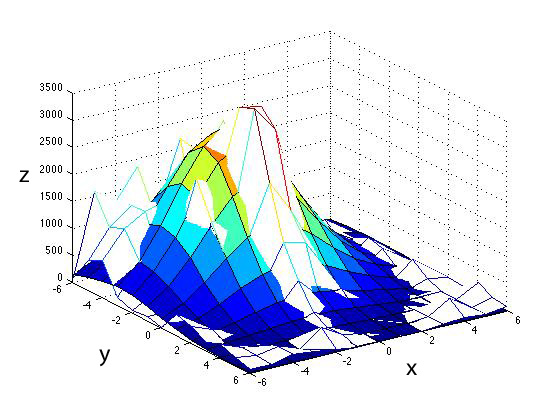
\includegraphics[scale=0.5]{\docroot results/figs/slide5}
\caption[Depiction of cluster detection]{Depiction of cluster detection. X and Y axes are pixels, with the Z axis being the grey level of the image. The white surface with coloured lines is a plot of what the script thinks might be a cluster, and the coloured surface with black lines is a plot of the best fitting 2D gaussian.}
\label{fig:imageprocessing:clusterdetection}
\end{center}
\end{figure}

\begin{figure}
\begin{center}
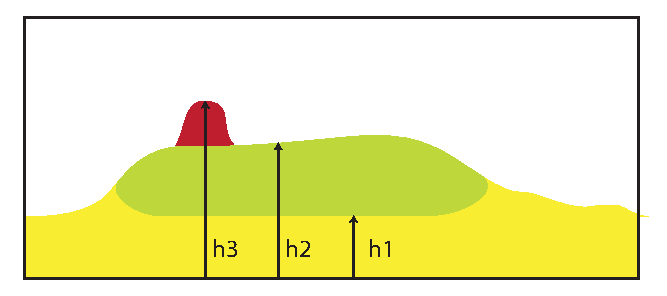
\includegraphics[width=0.7\textwidth]{\docroot results/figs/cellsideview.eps}
\caption[Side view of cell in image processing]{This figure shows a representation of the side view of a cell as considered by the image processing scripts. The yellow portion is identified as background level, the green portion as the cell, and the red portion as a cluster in the cell. The background level (h3) is estimated across the entire image and subtracted pixel for pixel. Similarly, an estimate of the height of the cell (h3-h2) is estimated below the cluster and subtracted pixel for pixel from the cluster (h1). This gives a zero base for the cluster, essential for cluster fitting.

Calculating the CheZ fraction is now simple; it is simply the volume of the red portion divided by the volume of the red an green portions combined.}
\label{figs:improc:sideview}
\end{center}
\end{figure}


A visual representation of the resulting masks and locations is shown in Figure~\ref{fig:imageprocessing:output}, in a system implemented for debugging.

\begin{figure}
\begin{center}
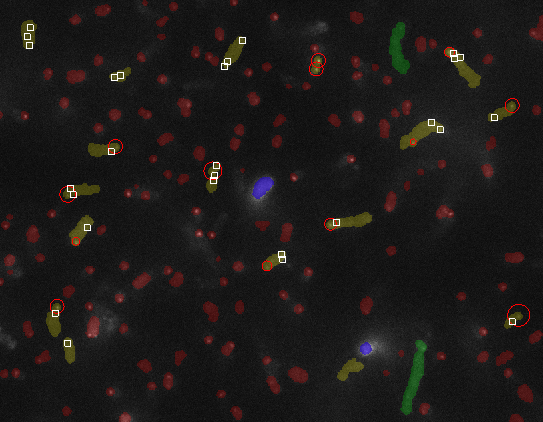
\includegraphics[width=0.8\textwidth]{\docroot results/figs/withcobalt-data.png}
\caption[Image Processing Output]{Image processing output. Yellow cells are cells that were identified by the cell finder and passed all conditions. Red cells failed from being too round. Blue cells failed from being too bright. Green cells failed from being too long. Red circles identify clusters that were identified by the cluster finder and passed all conditions, with the size of the circle being proportional to the size of the cluster. White squares identify clusters detected by the cluster finder but which failed on one or more condition. Image is from dataset as presented later in Figure~\ref{fig:results:nikon}.}
\label{fig:imageprocessing:output}
\end{center}
\end{figure}

\subsubsection{Image Alignment}

The OptoSplit II provided by Cairn Research allows for viewing two channels on the same sensor simultaneously. However, as the two images are adjacent in the same file, they must be split into two separate aligned images so that they may be accurately overlaid. This can be automated using some fairly simple mathematical methods.

The two images are extracted with a \(\simeq10\%\) safety border. A mean is taken of each image in each of the x and y axes. A least-squares fitted straight line mean is subtracted from each to negate the effect of any gradient across the image. Each pair of means is then aligned by gradient descent of the root mean square of the difference between them.

This provides the six data points required to align all future images taken until the OptoSplit II is adjusted again - the size of the image, and both of the locations.

Again, all scripts are available online, see appendix~\ref{sec:scripts:anisotropy}.

\newpage
\subsection{CheZ Fraction using Image Processing}

Calculating the CheZ fraction (the fraction of CheZ that is located in the chemotactic cluster as a proportion of all the CheZ in the cell) is a direct way to monitor the localisation of CheZ. As we are expecting an increase in CheZ clustering in response to an increase in repellent, we should see a corresponding increase in the CheZ fraction.

In each experiment, cultures of each strain were grown, induced and prepared for microscopy with and without \ce{CoSO4}, a repellent. Multiple images were taken of each, and run through the image processing described in section~\ref{sec:results:imageprocessing}.

Cells shown here are KL1005; \textsl{\(\Delta\)RBYZ)} with YFP tagged CheZ and mCherry tagged CheY. Removal of CheR and CheB removes the methyl adaptation system. Removal of CheZ and replacement with YFP tagged CheZ helps maintain the stoichiometry of the system. As a result of the natural arrangements of the operon no \textsl{\(\Delta\)RBZ} strain exists and so CheY has to be re-introduced too, as it is required in the proposed mechanism for CheZ cluster formation. CheZ-eYFP is an N-terminal fusion as this is believed to be less disruptive than C-termain fusions to oligomerisation.

\subsubsection{Epifluorescence Microscopy}
\label{sec:results:cs:epi}

These experiments were performed on a Nikon microscope on loan from the manufacturer. One image was taken each from a slide of cells prepared with and without \ce{CoSO4}. Data shown in Figure~\ref{fig:results:nikon}.

\begin{figure}
\begin{center}
\subfloat[No cobalt, \(n=18, \mu=0.144, \sigma=0.070\)]{
	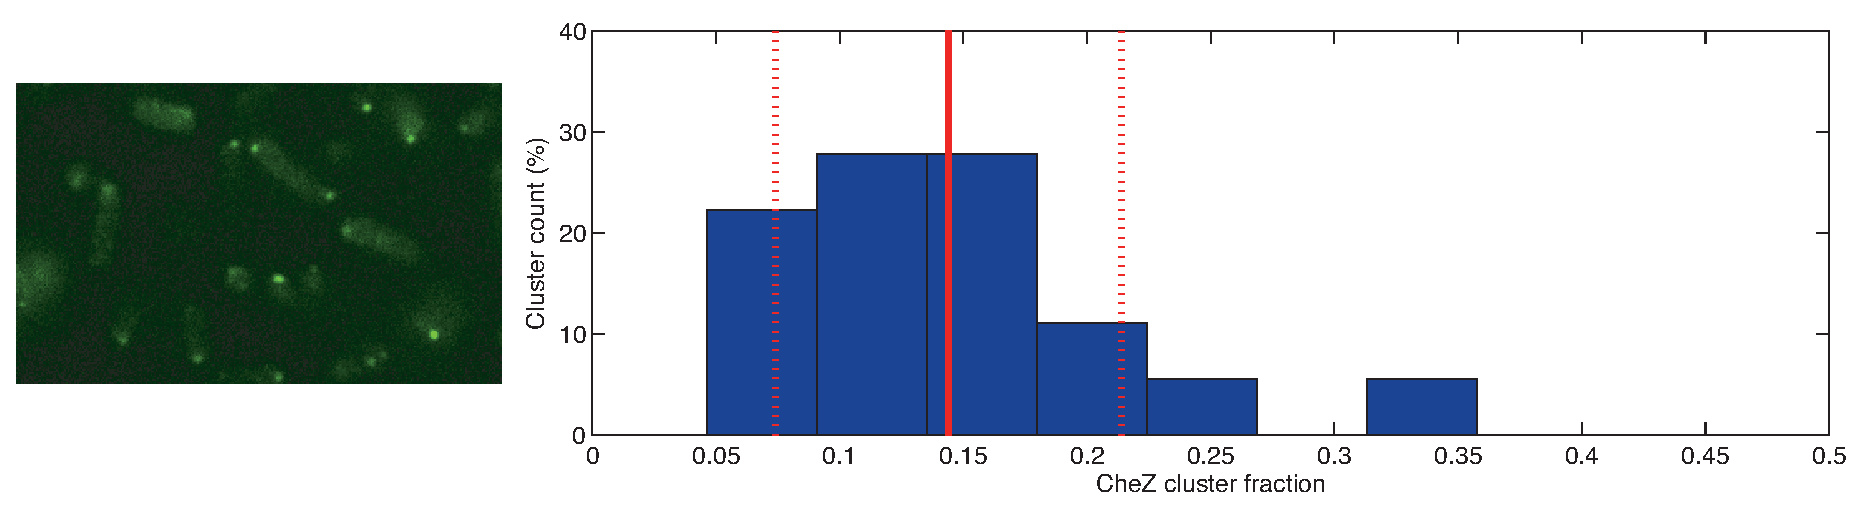
\includegraphics[width=\textwidth]{\docroot results/figs/nikon-nocob.eps}
	\label{fig:results:nikon:nocobalt}
}\\
\subfloat[With \SI{2}{\milli\Molar} \ce{CoSO4}, \(n=36, \mu=0.205, \sigma=0.116\)]{
	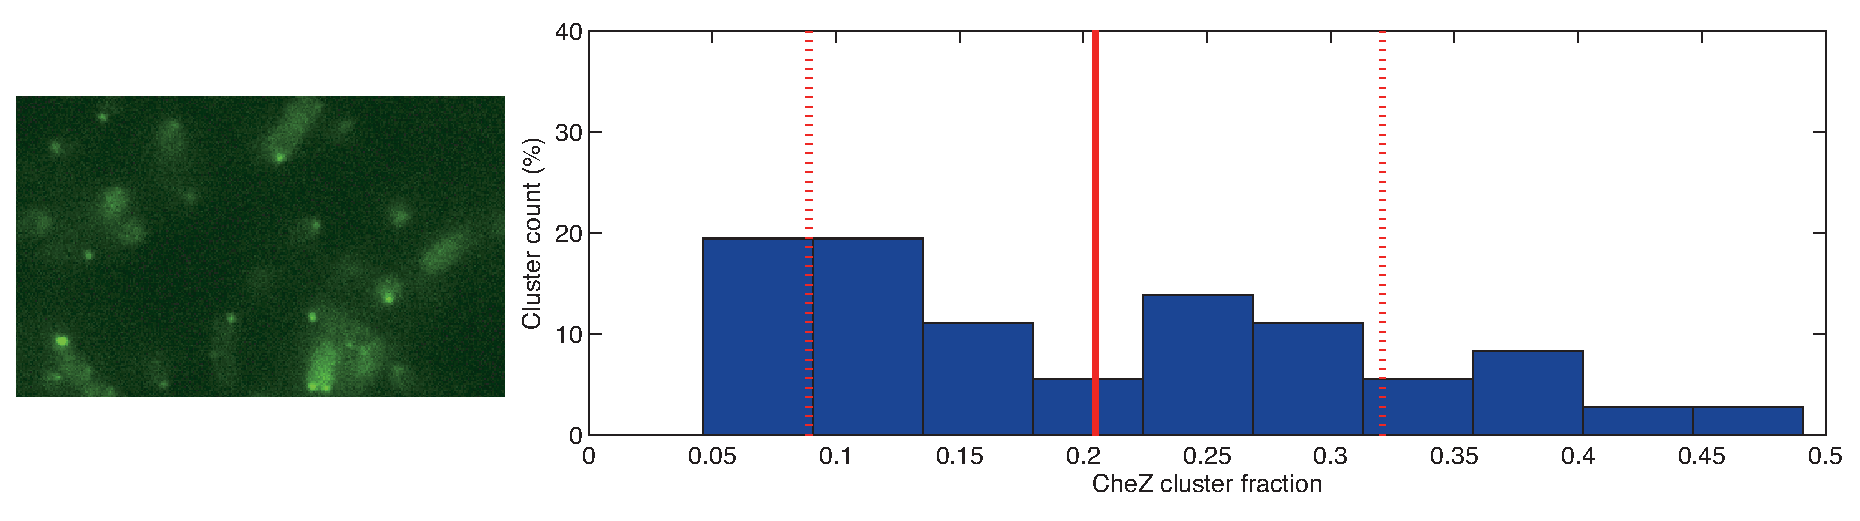
\includegraphics[width=\textwidth]{\docroot results/figs/nikon-cob.eps}
	\label{fig:results:nikon:cobalt}
}
\caption[Image processing results on Nikon microscope]{Histograms of CheZ cluster fraction (fraction of CheZ protein in cell localised in the polar cluster). Solid red line marks mean average, dashed lines \(\pm\sigma\). \(p\) value \(=4.4\%\) using the Student's t-test. Microscope: Nikon Ti-E widefield (demo). Strain: KL1005 \textsl{\(\Delta\)RBYZ, CheZ-eYFP, CheY-mCherry}.}
\label{fig:results:nikon}
\end{center}
\end{figure}

\subsubsection{Confocal Microscopy}
\label{sec:results:cs:confocal}
These experiments were performed on a Zeiss confocal microscope, the use of which was kindly given to us by Alessandro Esposito at the Hutchison MRC. Ten images were taken each from a slide of cells prepared with and without cobalt. Data shown in Figure~\ref{fig:results:zeiss}.

\begin{figure}
\begin{center}
\subfloat[No cobalt, \(n=1222, \mu=0.185, \sigma=0.068\)]{
	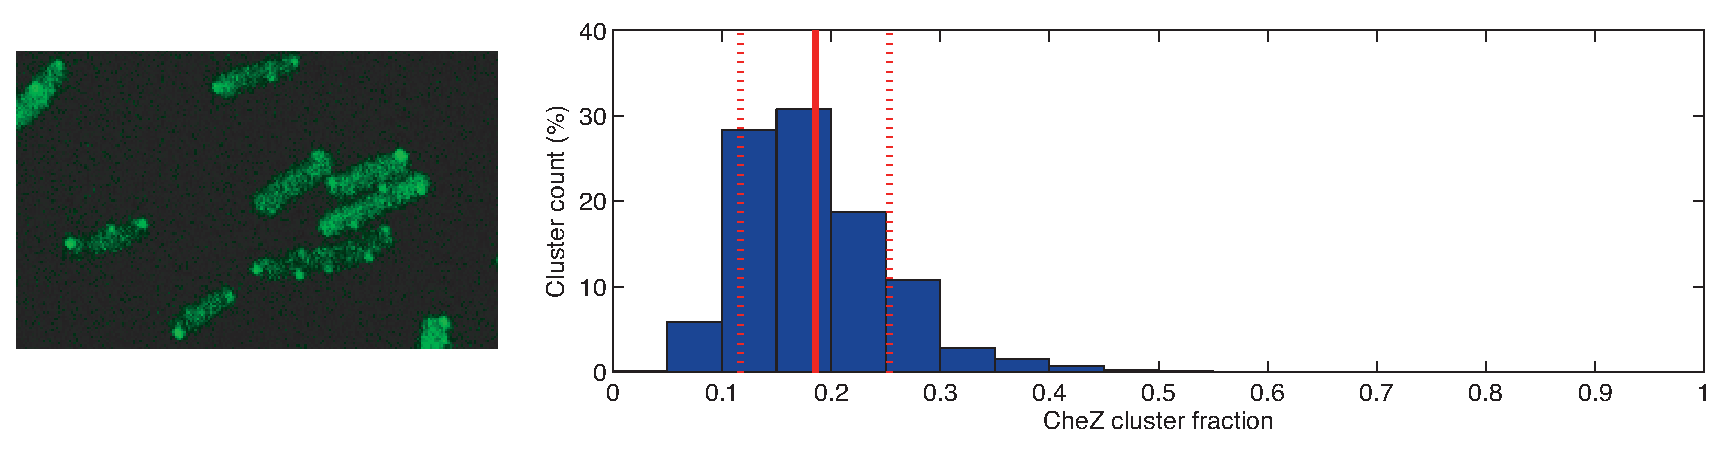
\includegraphics[width=\textwidth]{\docroot results/figs/zeiss-nocob.eps}
	\label{fig:results:zeiss:nocobalt}
}\\
\subfloat[With \SI{2}{\milli\Molar} \ce{CoSO4}, \(n=644, \mu=0.198, \sigma=0.082\)]{
	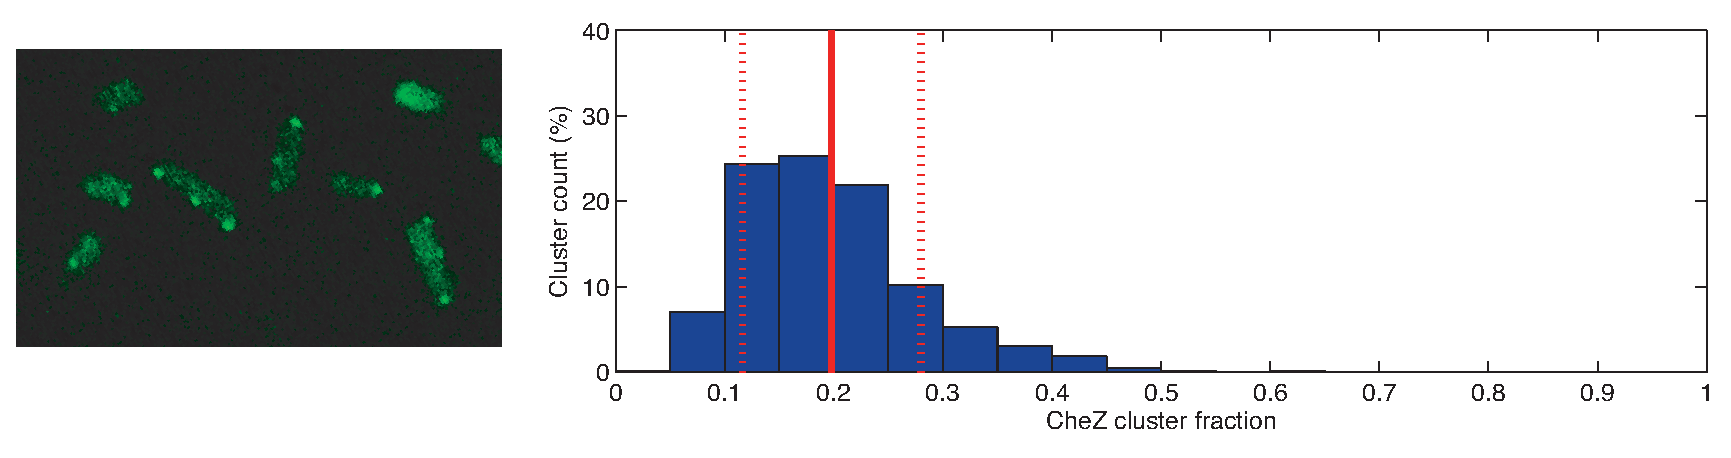
\includegraphics[width=\textwidth]{\docroot results/figs/zeiss-cob.eps}
	\label{fig:results:zeiss:cobalt}
}
\caption[Image processing results on Zeiss confocal microscope]{Histograms of CheZ cluster fraction (fraction of CheZ protein in cell localised in the polar cluster). Solid red line marks mean average, dashed lines \(\pm\sigma\). \(p\) value \(=0.0349\%\) using the Student's t-test. Microscope: Zeiss confocal. Strain: KL1005 \textsl{\(\Delta\)RBYZ, CheZ-eYFP, CheY-mCherry}.}
\label{fig:results:zeiss}
\end{center}
\end{figure}

\cleardoublepage

\subsection{Fluorescent Proteins}

Primarily EYFP was used for the proteins being imaged. However, a monomeric form was required for anisotropy~\citep{vaknin07}. This is achieved through the A206K mutation. Another monomeric EYFP variant, known as Venus and also containing the A206K mutation, was described as being a better FRET receiver~\citep{nagai02} as well as a generally improved fluorophore, and therefore ideal for our homo-FRET experiments. However, only the monomeric (A206K) EYFP variant was available to us.

Site directed mutagenesis was initially to be used to create the mutations from EYFP to Venus, but this was not followed through due to cost and also after receiving what was described as Venus, but which, after sequencing, turned out to be EYFP with the A206K mutation.

Primers for standard cloning with multiple restriction sites were designed (see appendix~\ref{sec:plaspri}); however, after repeated cloning attempts we failed to obtain a final construct, and after several weeks this assembly method was abandoned.

With kind support from other sources (see appendix~\ref{sec:plaspri:plas}) we built up a library of many fluorescent protein-chemotaxis protein fusions. However, it was still necessary to exchange many of these. Many fluorescent proteins (e.g. CFP, YFP, BFP) are derivatives of GFP through only a few amino acid substitutions~\citep{tsien98}. In most modernly used GFP derivatives, these all lie between amino acid 64 and amino acid 206, inclusive. Therefore, through careful design of PCR primers Gibson assembly can be used to exchange one GFP derivative for another with the same set of primers (see appendix~\ref{sec:plaspri:pri}).

Gibson assembly worked on the first time, and was used with a perfect success rate for all subsequent exchanges. Backbones were split in to two to ensure that PCR would be able to run their entire length. Whilst each of the five PCR reactions had a lot of misprimes and over-extensions, the desired bands were strong enough to be easily visible, and after gel extraction specific enough to perform Gibson assembly successfully (Figure~\ref{fig:results:gibson}). After transformation, all assemblies were sequenced. All showed the A206K mutation and no other changes to the coding sequence.

\begin{figure}
\begin{center}
\subfloat[pET-AS]{
	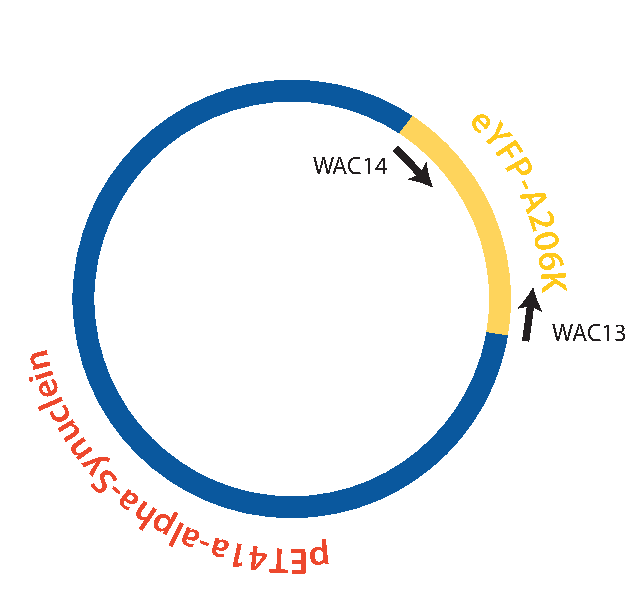
\includegraphics[width=0.35\textwidth]{\docroot results/figs/A206K}
	\label{fig:results:gibson:A206K}
}
\subfloat[pVS49]{
	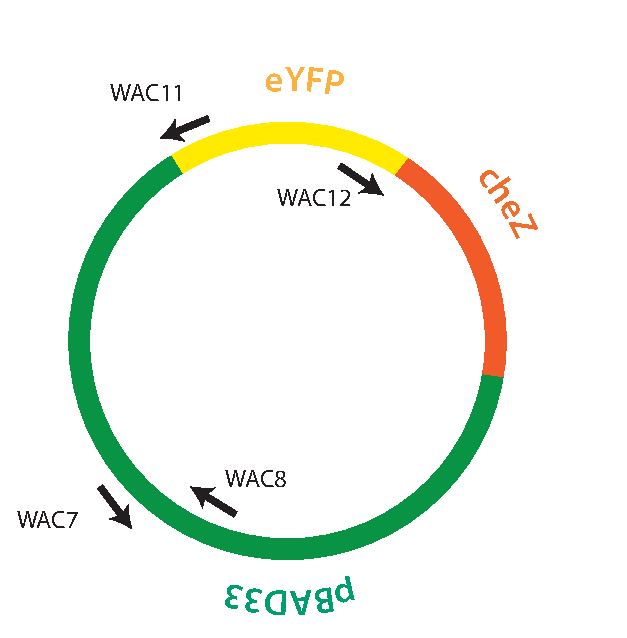
\includegraphics[width=0.35\textwidth]{\docroot results/figs/pVS49split}
	\label{fig:results:gibson:49}
}
\subfloat[pVS289]{
	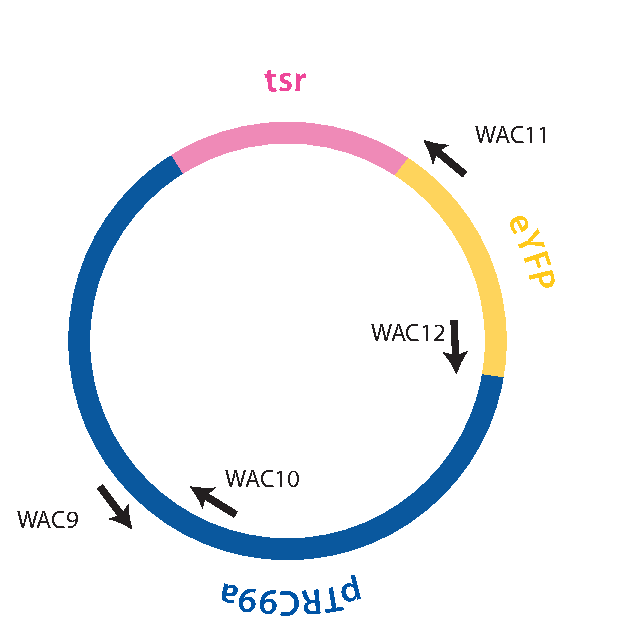
\includegraphics[width=0.35\textwidth]{\docroot results/figs/pVS289split}
	\label{fig:results:gibson:289}
}
\\
\subfloat[PCR Gel]{
	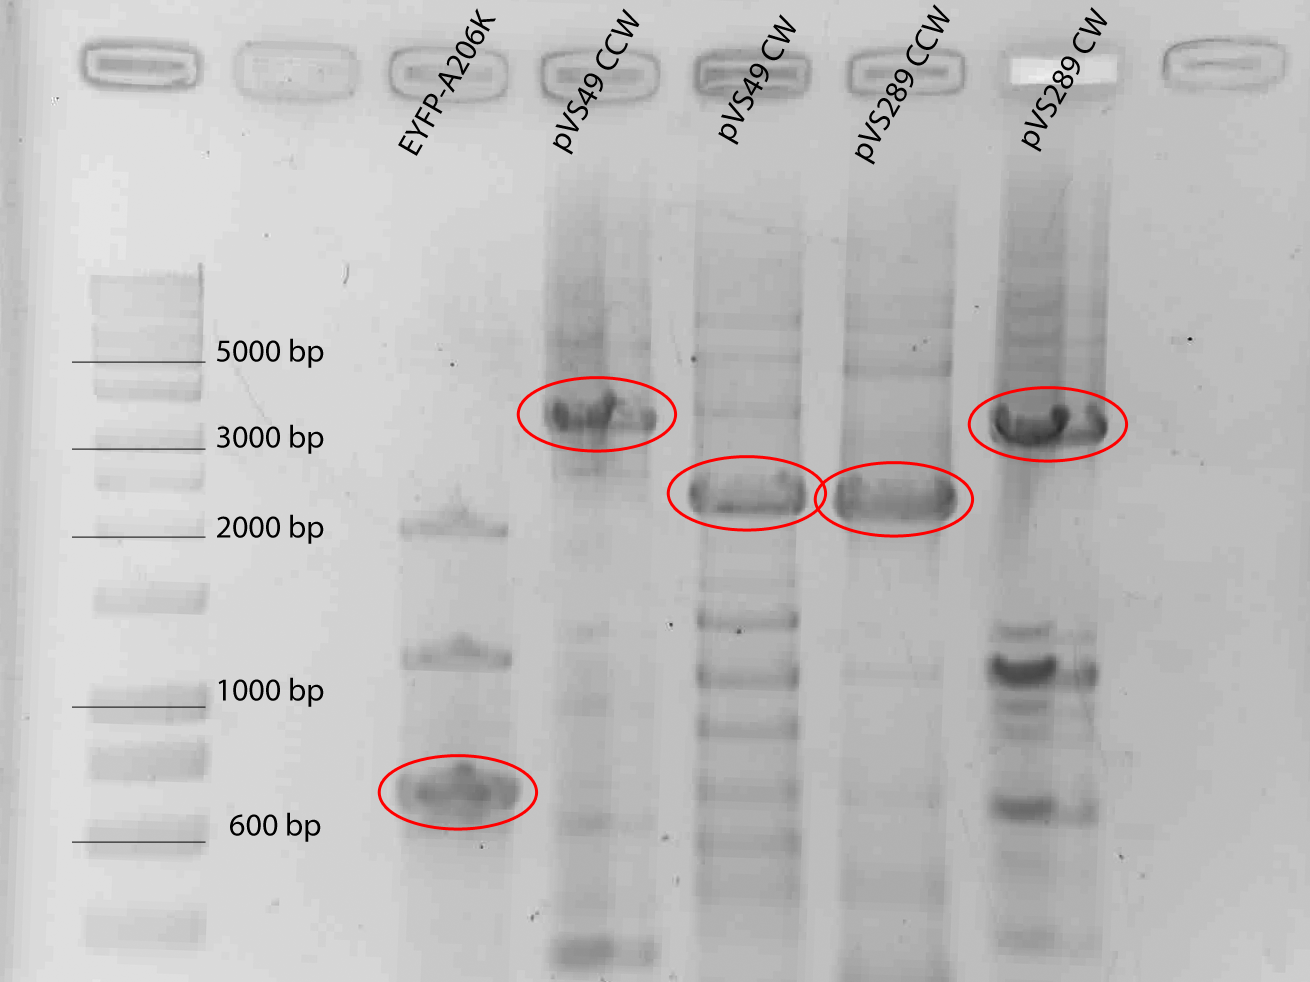
\includegraphics[width=0.7\textwidth]{\docroot results/figs/gibsonpcr.png}
	\label{fig:results:gibson:pcr}
}
\caption[PCR results for Gibson Assembly]{PCR to create overlaps for Gibson Assembly. \subref{fig:results:gibson:A206K}, \subref{fig:results:gibson:49} and \subref{fig:results:gibson:289}: schematics of plasmid templates. \subref{fig:results:gibson:pcr}: agarose gel of PCR products, with desired bands circled in red. pWAC1 was created by Gibson Assembly from circled, gel purified bands from lanes 3, 4 and 5; pWAC4 from lanes 3, 5 and 6.}
\label{fig:results:gibson}
\end{center}
\end{figure}
\newpage

\subsection{Microfluidics}

In order to obtain live imaging of the response to chemotactic chemicals, we must be able to replace the media in which the cells are contained with media of differing concentrations of attractant or repellent. Inspired by Howard Berg and Steven Block's work~\citep{berg84} we set out to create a microfluidics flow cell that would allow for precise exchange of media. Aladdin pumps from WPI-Europe were used due to their relatively well documented scripting capabilities and economy - precision was not as pressing concern as normally found in microfluidic applications. Two different microfluidic devices are required.

\begin{figure}[h!]
\begin{center}
\subfloat[Simple microfluidics device for step changes]{
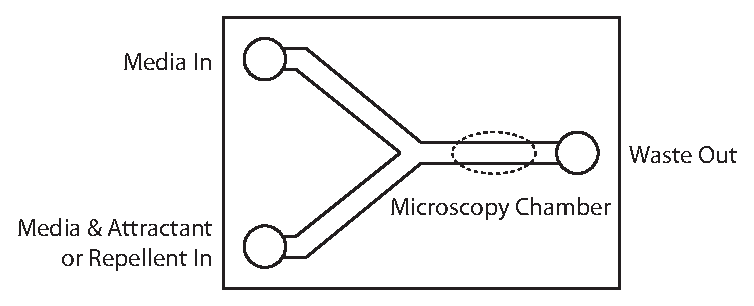
\includegraphics[scale=1]{\docroot results/figs/simplemicrofluidic.eps}
\label{fig:microfluidics:simple}
}\\
\subfloat[Complex microfluidics device for smooth mixing]{
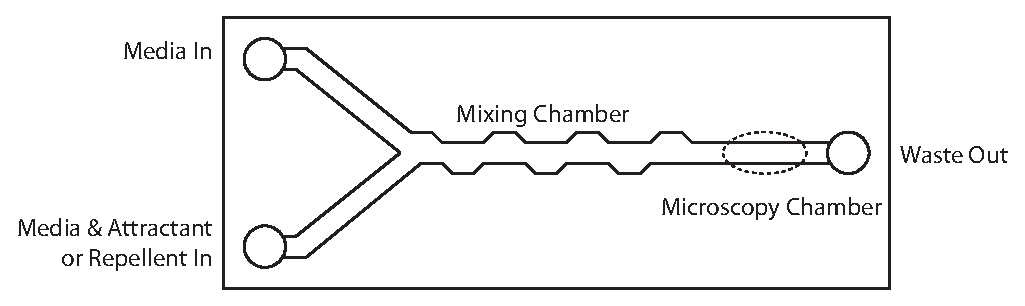
\includegraphics[scale=1]{\docroot results/figs/complexmicrofluidic.eps}
\label{fig:microfluidics:complex}
}
\caption[Microfluidics devices]{Schematics (not to scale) representative of the two types of microfluidics devices planned. The channels (parallel lines) are about \SI{1}{\milli\meter} wide and \SI{100}{\micro\meter} deep.}
\label{fig:microfluidics}
\end{center}
\end{figure}

The first, in Figure~\ref{fig:microfluidics:simple}, is a simple Y shaped splitter with only one syringe active at any time. One syringe will be filled with a plain buffer, and the other with buffer with attractant/repellent at a set concentration. This allows for rapid switching on and off of the attractant/repellent.

The second, in Figure~\ref{fig:microfluidics:complex}, is a more complex splitter to allow for thorough mixing of the two inputs. This takes the form of a zig-zag style channel between the two inputs and the chamber containing bacteria. Again, one syringe would be filled with a plain media, and the other with media with attractant/repellent at a set concentration. By varying the relative rates of the two pumps but keeping the total constant, the concentration of attractant/repellent can be varied between zero and the aforementioned concentration. A potential drawback of this system is firstly the lag between changing pump speeds and observing a change in concentration in the bacterial chamber, and secondly the smoothing of a step change in concentration due to forward and backward diffusion of the attractant/repellent.

We received flow cells of the design in Figure~\ref{fig:microfluidics:simple} constructed from PDMS, bonded to \(\sim\)\SI{1}{\milli\meter} PDMS, from Fabrice Gielen, Hollfelder Group, Department of Biochemistry. We found that a deposit of live cells could be stuck to the inside surface of the flow cells by flushing them through with first poly-L-lysine, then blank media, then the cells, and finally blank media again.

\subsection{Inducer Calibration}

Most fusion proteins were available, or could easily be made available, in both the pBAD33 or pTRC99a plasmid, induced by arabinose or IPTG respectively. As in some experiments we planned to induce two proteins, one from each plasmid, it was important to be able to balance the production of each, by performing titrating the inducer concentration. The expression of \textsl{CheZ-eYFP} was monitored in two strains, KL1001 and KL1019, induced by Arabinose and IPTG respectively (for details, see appendix~\ref{sec:plaspri}).

Images are shown of each of four different concentrations of inducer \SI{3.5}{\hour} after induction in each strain.

\begin{figure}
\begin{center}
\subfloat[0.001\% Arabinose]{
	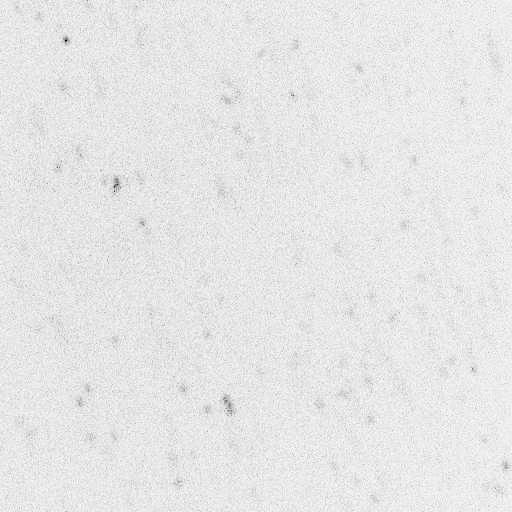
\includegraphics[width=.45\linewidth]{\docroot results/figs/A1-yfp.jpg}
}
\subfloat[0.005\% Arabinose]{
	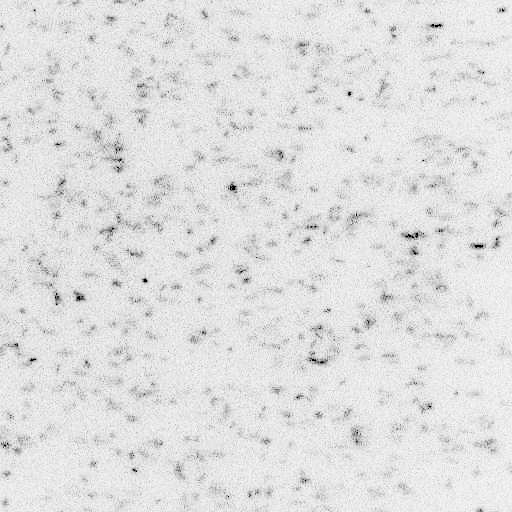
\includegraphics[width=.45\linewidth]{\docroot results/figs/A2-yfp.jpg}
}\\
\subfloat[0.01\% Arabinose]{
	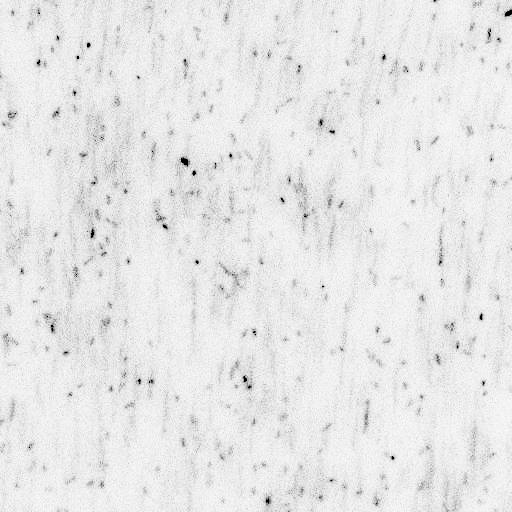
\includegraphics[width=.45\linewidth]{\docroot results/figs/A3-yfp.jpg}
}
\subfloat[0.05\% Arabinose]{
	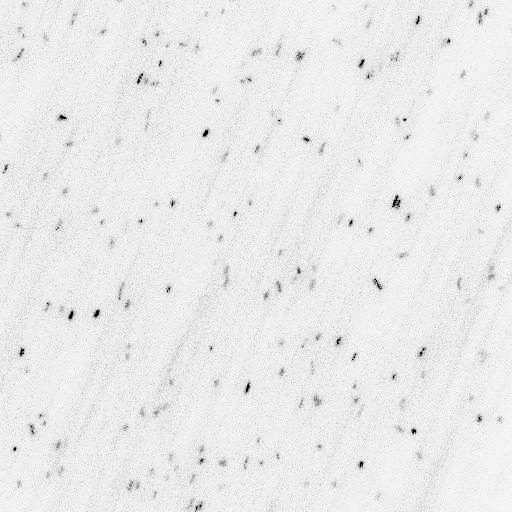
\includegraphics[width=.45\linewidth]{\docroot results/figs/A4-yfp.jpg}
}
\caption[Arabinose inducer titration]{Arabinose inducing \textsl{CheZ-eYFP} expression in KL1001. Colours inverted to improve printed contrast. Microscope: Nikon Ti-E with 40X 0.60NA objective.}
\end{center}
\end{figure}

\begin{figure}
\begin{center}
\subfloat[\SI{5}{\micro\Molar} IPTG]{
	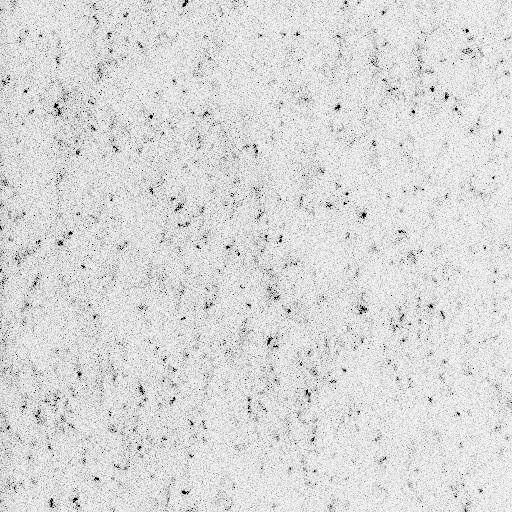
\includegraphics[width=.45\linewidth]{\docroot results/figs/S5-yfp.jpg}
}
\subfloat[\SI{10}{\micro\Molar} IPTG]{
	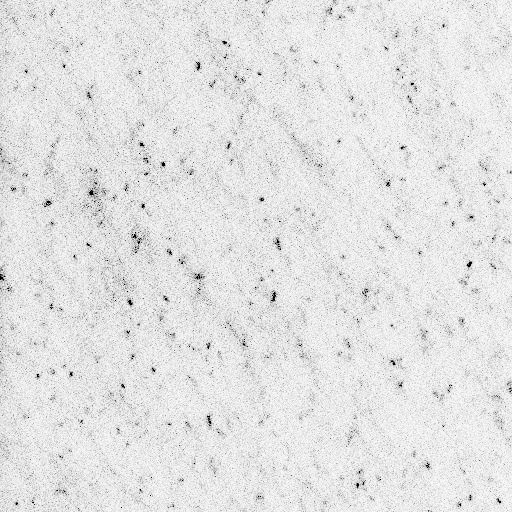
\includegraphics[width=.45\linewidth]{\docroot results/figs/S6-yfp.jpg}
}\\
\subfloat[\SI{20}{\micro\Molar} IPTG]{
	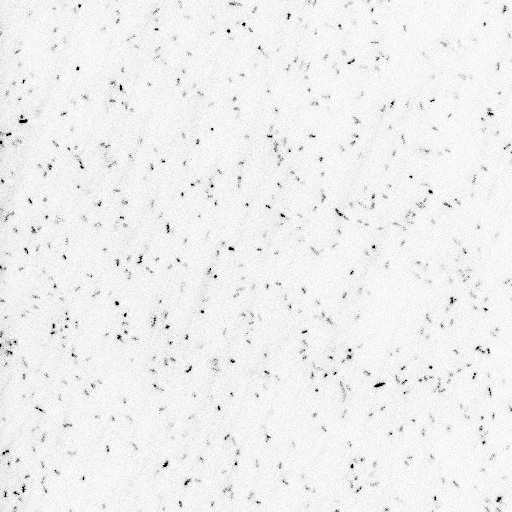
\includegraphics[width=.45\linewidth]{\docroot results/figs/S7-yfp.jpg}
}
\subfloat[\SI{40}{\micro\Molar} IPTG]{
	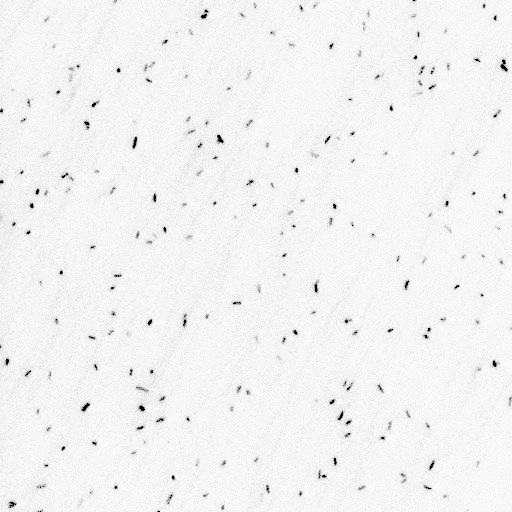
\includegraphics[width=.45\linewidth]{\docroot results/figs/S8-yfp.jpg}
}
\caption[IPTG inducer titration]{IPTG inducing \textsl{CheZ-eYFP} expression in KL1019. Colours inverted to improve printed contrast. Microscope: Nikon Ti-E with 40X 0.60NA objective.}
\end{center}
\end{figure}




\begin{comment}
\paragraph{Inducement time.} Generally it is recommended to induce some time after inoculating fresh media with overnight cultures; however this is not necessary if the proteins being induced are not toxic. Two parallel growths were done, OD measurements taken every two hours, and images recorded 4 hours after induction and four hours after inoculation.
\begin{center}
\begin{tabular}{ccc}
t=0	&	Inoculate	&	Inoculate \& Induce\\
2	&	Induce	&\\
4	&	Image	&	Image\\
6	&	Image	&
\end{tabular}
\end{center}

\paragraph{Inducer Titre} A logarithmic course of inducer concentrations was checked for expression of the same fusion protein under different promoters.

\begin{center}
\begin{tabular}{cc}
\textbf{Arabinose}	&	\textbf{IPTG} 	\\
0.001\%	&	\SI{1}{\micro\Molar}\\
0.003\%	&	\SI{3}{\micro\Molar}\\
0.01\%	&	\SI{10}{\micro\Molar}\\
0.03\%	&	\SI{30}{\micro\Molar}\\
0.1\%	&	\SI{100}{\micro\Molar}\\

\end{tabular}
\end{center}

\paragraph{Time Course}	A selection of inducer concentration from the inducer titre were re-run with samples being removed and imaged at \SI{2}{\hour}, \SI{3}{\hour} and \SI{4}{\hour} to find optimal expression.
 \end{comment}
\newpage
\subsection{Homo-FRET}
Some preliminary work has been done towards homo-FRET measurements. However, the microscopy system and cells require extensive calibration before good quantitative results can be taken. The Cairn OptoSplit must be set up to completely separate the two polarisations of light, and aligned to minimise distortion between the two images. As such, while some images have been taken they will not yield good quantitative results and so are not presented here.
\end{document}